\section{问题二的模型建立与求解}

\subsection{模型建立}

问题二使用第0--2399小时实际任务和逐时电力参数重新优化执行区域与开工时刻，预测结果不参与调度；第2400--2405小时仅用于收尾和结算，任务须在2406前完成。本问不考虑储能。
碳感知数据中心研究表明，电力碳强度可以作为任务调度和能源管理的重要决策信号\cite{ref5}；
跨区域负荷迁移能够利用不同区域的电力与碳排放差异，
但同时会引入网络时延和服务质量代价\cite{ref6}。
据此在任务时限、网络时延、GPU及功率约束下评价成本、碳排放、通信时延和新能源利用率。

任务参数及跨小时占用沿用问题一；实时任务立即开工，弹性任务可在合法时窗内错峰。
设$x_{irs}$表示任务$i$是否在区域$r$、时刻$s$开工，
候选区域$R_i$满足网络时延限制，
候选开工集合$S_i$满足到达时间、完成期限及2406终端约束。

设区域$r$在时刻$t$的AI IT负荷、总IT负荷和设施负荷分别为
$P^{AI}_{rt}$、$P^{IT}_{rt}$和$F_{rt}$。
利用问题一式(\ref{eq:q1_overlap})中的跨小时占用比例，有
\begin{equation}
	\begin{aligned}
		P^{AI}_{rt}
		&=
		\sum_i\sum_{s\in S_i}
		p_i\rho_{ist}x_{irs},\\
		P^{IT}_{rt}
		&=
		P^{NonAI}_{rt}+P^{AI}_{rt},\\
		F_{rt}
		&=
		PUE_rP^{IT}_{rt}.
	\end{aligned}
	\label{eq:q2_load_mapping}
\end{equation}

逐时GPU占用仍满足问题一约束。将IT容量、设施容量和最大购电能力合并为有效AI IT容量
$\bar P^{AI}_{rt}
=\min\{P^{IT,\max}_{rt}-P^{NonAI}_{rt},
P^{Facility,\max}_{rt}/PUE_r-P^{NonAI}_{rt},
(P^{RE}_{rt}+P_r^{Grid,\max})/PUE_r-P^{NonAI}_{rt}\}$，
并要求$P^{AI}_{rt}\leq\bar P^{AI}_{rt}$；其余GPU、时延和时限约束沿用问题一。

无储能时，新能源优先供给本地负荷，不足由电网补充，富余部分按上限外送，其余弃用。
设$V_{rt}$、$B_{rt}$、$X_{rt}$和$R_{rt}$分别为
新能源直接消纳、电网购电、新能源外送和弃用功率，则
\begin{equation}
	\begin{aligned}
		V_{rt}&=\min(F_{rt},P^{RE}_{rt}),\\
		B_{rt}&=\max(F_{rt}-P^{RE}_{rt},0),\\
		X_{rt}&=\min\{\max(P^{RE}_{rt}-F_{rt},0),\bar X_r\},\\
		R_{rt}&=P^{RE}_{rt}-V_{rt}-X_{rt},
	\end{aligned}
	\label{eq:q2_energy}
\end{equation}
其中$0\leq B_{rt}\leq P_r^{Grid,\max}$，$0\leq X_{rt}\leq\bar X_r$。

以净运行成本$C$、碳排放$E$、平均网络时延$L$
和新能源利用率$U$评价方案。
在$t=0,\ldots,2405$上定义
\begin{equation}
	\begin{aligned}
		C
		&=
		\sum_r\sum_{t=0}^{2405}
		\left(\pi_{rt}B_{rt}-\sigma_{rt}X_{rt}\right),\\
		E
		&=
		\sum_r\sum_{t=0}^{2405}\kappa_{rt}B_{rt},\\
		L
		&=
		\frac{1}{N}
		\sum_i\sum_{r\in R_i}\sum_{s\in S_i}
		l_{ir}x_{irs},\\
		U
		&=
		\frac{\displaystyle
			\sum_r\sum_{t=0}^{2405}(V_{rt}+X_{rt})}
		{\displaystyle
			\sum_r\sum_{t=0}^{2405}P^{RE}_{rt}},
		\qquad Q=1-U.
	\end{aligned}
	\label{eq:q2_objectives}
\end{equation}

令$f_1=C,f_2=E,f_3=L,f_4=Q$。分别求解单目标连续松弛得到理想下界$f_m^{LB}$，再结合纯算力基准$f_m^0$和单目标锚点$x^{(a)}$建立固定尺度：
\begin{equation}
	\begin{aligned}
		f_m^{ref}
		&=
		\max\left\{
		f_m^0,\max_a f_m(x^{(a)})
		\right\},\\
		R_m
		&=
		f_m^{ref}-f_m^{LB},\\
		d_m(x)
		&=
		\frac{f_m(x)-f_m^{LB}}{R_m},\\
		\min\quad z,
		&\qquad d_m(x)\leq z,\quad \forall m .
	\end{aligned}
	\label{eq:q2_minmax}
\end{equation}

若$R_m\approx0$，该指标仅用于结果评价；否则式(\ref{eq:q2_minmax})最小化最大标准化偏离。

多时间尺度滚动常用于处理任务到达、负荷和能源状态的动态耦合\cite{ref7}，低碳在线调度还需协调服务质量与能源指标\cite{ref8}。针对50000个任务，本文采用$H=24$ h决策窗口、$K=48$ h前瞻窗口，结合可行性修复和局部混合整数线性规划精修。
在滚动起点$\tau$，
考察$[\tau,\tau+H+K)$范围，
但仅固定$[\tau,\tau+H)$内实际开工任务；
已开工任务保持原安排，
最晚合法开工时刻进入当前窗口的弹性任务必须在本轮开工。

构造阶段先安排实时任务，再按时间裕量和资源需求排序处理弹性任务。
定义当前全时域目标估计
$\hat f_{m,\tau}
=f_m^0+\Delta f_{m,\tau}^{past}
+f_{m,\tau}^{scope}-f_{m,\tau}^{0,scope}$。
对合法候选$(r,s)$计算
\begin{equation}
	S_{irs}
	=
	\max_m
	\left\{
	\frac{
		\hat f_{m,\tau}
		+\Delta f_{m,irs}
		-f_m^{LB}}
	{R_m}
	\right\},
	\qquad
	(r_i^*,s_i^*)
	=
	\arg\min_{(r,s)}S_{irs}.
	\label{eq:q2_marginal}
\end{equation}

若出现容量冲突则重排可替代任务；得到可行解后选择关键任务形成大邻域，并固定邻域外决策进行精修，流程见表\ref{tab:q2_algorithm}。

\begin{table}[H]
	\centering
	\caption{问题二滚动数学启发式求解流程}
	\label{tab:q2_algorithm}
	
	\fontsize{10.5pt}{12pt}\selectfont
	\renewcommand{\arraystretch}{0.88}
	
	\begin{tabular}{
			>{\centering\arraybackslash}p{0.08\textwidth}
			>{\raggedright\arraybackslash}p{0.86\textwidth}}
		\toprule
		\textbf{步骤} & \multicolumn{1}{c}{\textbf{主要操作}}\\
		\midrule
		
		1 &
		由连续松弛、问题二纯算力基准及单目标锚点确定固定定标尺度。\\
		
		2 &
		读取$H=24$ h决策窗口与$K=48$ h前瞻区，
		锁定已开工任务并识别本轮必须开工任务。\\
		
		3 &
		实时任务立即安排；弹性任务按时间裕量和资源需求排序，
		利用式(\ref{eq:q2_marginal})选择可行候选。\\
		
		4 &
		更新GPU、AI IT负荷和能源状态；
		出现容量冲突时重新安排可替代任务。\\
		
		5 &
		选择关键任务形成大邻域，
		固定邻域外方案并利用小规模混合整数线性规划模型精修。\\
		
		6 &
		提交当前$H$小时决策并继续滚动；
		最终重构0--2405小时全时域剖面并独立核验。\\
		
		\bottomrule
	\end{tabular}
\end{table}


该方法按原多目标准则评价候选，数学启发式仅缩小整数搜索范围；所得结果为严格满足硬约束且计算效率较高的可行方案，不宣称获得全局最优解。


\subsection{求解结果与模型检验}

按问题一原则构造50000个任务的全时域纯算力基准，并以问题二能源口径结算；滚动求解结果见表\ref{tab:q2_result}。

% ==================== Q2：多目标结果 ====================
\begin{table}[H]
	\centering
	\caption{问题二多目标调度与问题二纯算力基准对比}
	\label{tab:q2_result}
	
	\fontsize{10.5pt}{12pt}\selectfont
	\renewcommand{\arraystretch}{0.90}
	
	\begin{tabular}{lccc}
		\toprule
		\multicolumn{1}{c}{\textbf{评价指标}}
		& \textbf{问题二纯算力基准}
		& \textbf{问题二均衡方案}
		& \textbf{变化}\\
		\midrule
		
		净运行成本/元
		& $-4.196834\times10^8$
		& $-4.247568\times10^8$
		& 降低507.34万元\\
		
		碳排放/tCO$_2$
		& 8.850562
		& 10.125791
		& 增加1.275228\\
		
		平均网络时延/ms
		& 5.000000
		& 12.946840
		& 增加7.946840\\
		
		新能源利用率
		& 67.91598\%
		& 68.13914\%
		& 提高0.22316个百分点\\
		
		平均等待时间/h
		& 0.00116
		& 30.89284
		& 增加30.89168\\
		
		跨区域迁移比例
		& 0
		& 29.35800\%
		& 增加29.35800个百分点\\
		
		\bottomrule
	\end{tabular}
\end{table}


表\ref{tab:q2_result}显示，净运行成本降低507.34万元、新能源利用率提高0.22316个百分点，但碳排放增加1.2752 tCO$_2$、平均网络时延增加7.95 ms；负成本表示外送收益超过购电支出。

固定定标后，纯算力基准四项偏离为1.00、1.00、0和1.00，问题二方案为0.85、1.14、1.15和0.87，最大偏离$z=1.15$。

\begin{figure}[H]
	\centering
	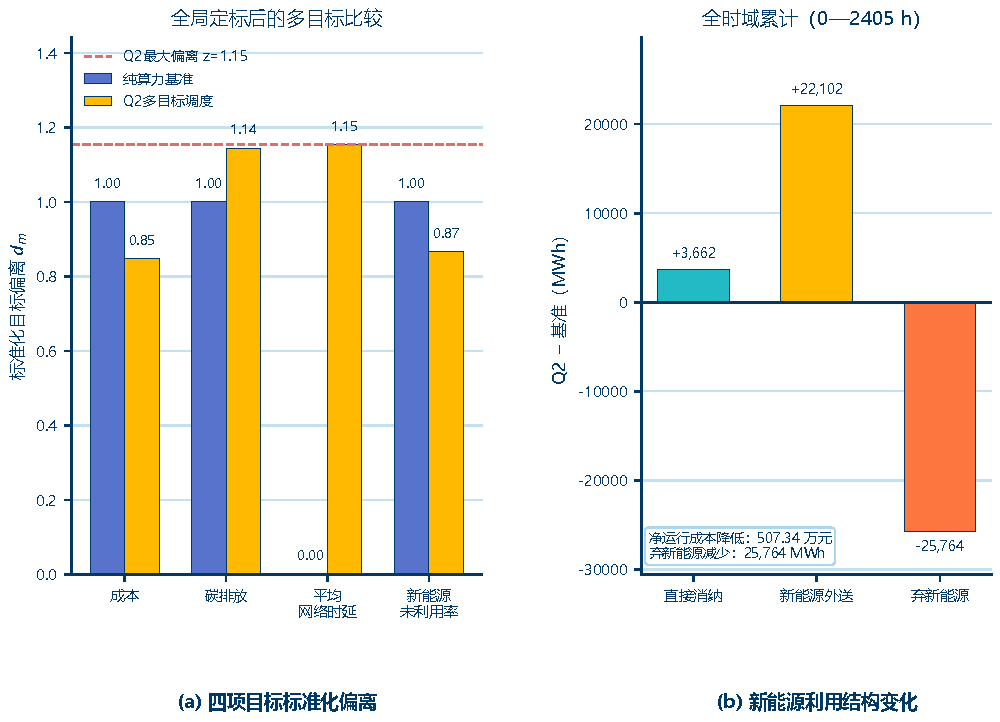
\includegraphics[width=0.82\textwidth]
	{figures/q2_group1_core_results.pdf}
	\caption{问题二多目标调度效果及新能源利用结构变化}
	\label{fig:q2_core}
\end{figure}

图\ref{fig:q2_core}中，新能源直接消纳、外送分别增加约3662、22102 MWh，弃用减少约25764 MWh，变化量基本闭合。

共有35321个任务本地执行、14679个跨区域迁移，迁移比例29.358\%，迁移GPU工作量为$1.308142\times10^6\,\mathrm{GPU\cdot h}$。

图\ref{fig:q2_migration}显示D、E、F迁出较多，C、D吸收较多跨区域算力，迁移方向同时受资源和能源条件影响。

依据50000条任务记录重构0--2405小时剖面，两方案累计量保持一致：AI IT能耗均为$7.389279853\times10^5$ MWh，GPU工作量均为$5.020787\times10^6$ GPU$\cdot$h；
任务、时延、时限、容量和购电边界均无违反，能源平衡残差为0，2406时点无任务占用。

91个精修窗口中45个接受改进，平均改善2.43\%。窗口0--9的同窗精确对照显示，中位计算速度提高约31.8倍，平均绝对相对偏差为39.82\%，最大标准化目标偏差为293.40\%。该最大值是局部窗口标准化目标的相对偏差，不等同于全时域成本、碳排放等指标的整体误差，但表明受限邻域在个别资源紧张窗口中可能遗漏更优的任务组合。因此，本文仅将其作为能够严格满足硬约束的大规模近似求解方法，不宣称获得局部或全时域最优解。

\begin{figure}[H]
	\centering
	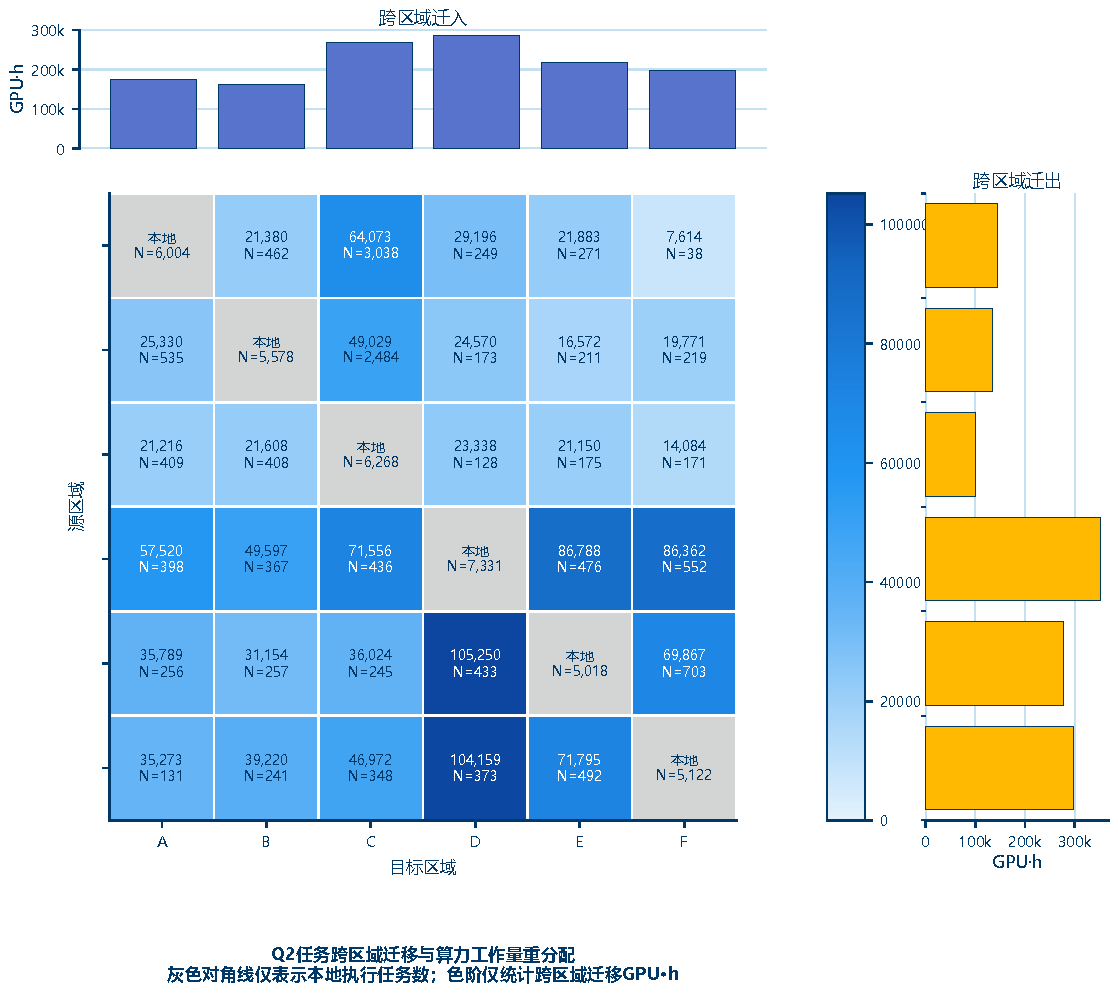
\includegraphics[width=0.68\textwidth]
	{figures/q2_group2_dispatch_mechanism.pdf}
	\caption{问题二任务跨区域迁移与算力工作量重分配}
	\label{fig:q2_migration}
\end{figure}

\begin{figure}[H]
	\centering
	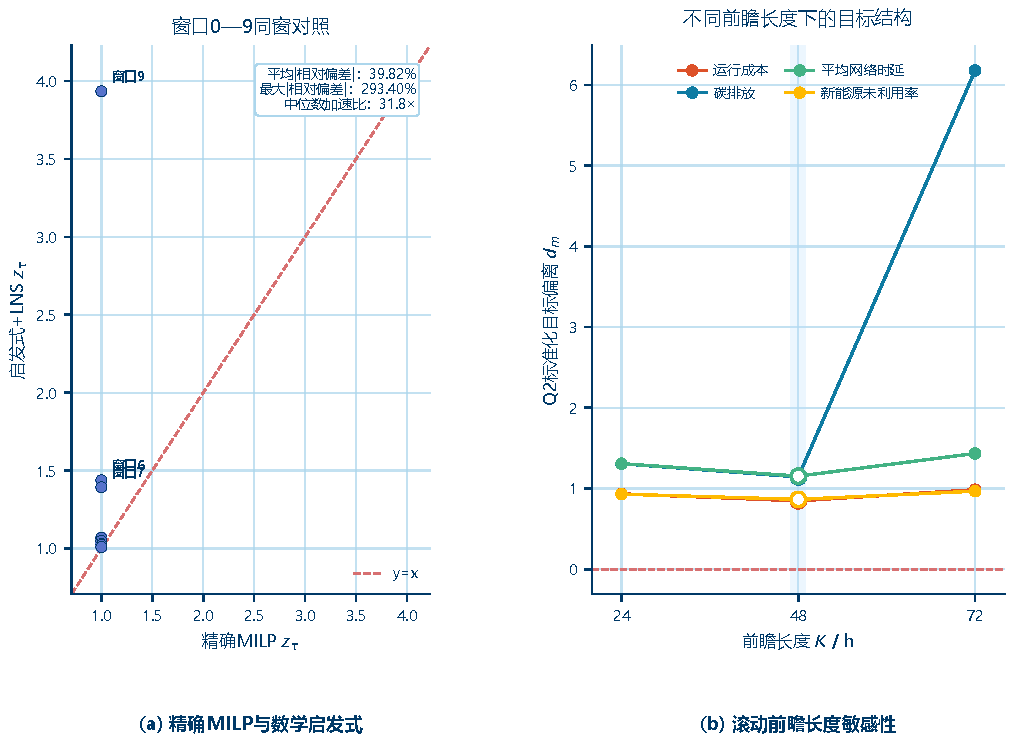
\includegraphics[width=0.72\textwidth]
	{figures/q2_group3_model_validation.pdf}
	\caption{问题二数学启发式求解质量与前瞻长度敏感性}
	\label{fig:q2_validation}
\end{figure}

前瞻长度检验中，$K=24$ h与48 h的目标结构接近，$K=72$ h仅使碳排放明显增大，故采用$H=24$ h、$K=48$ h。

问题二以碳排放、网络时延和等待增加换取成本降低与新能源利用提高，全时域复算满足硬约束，可作为问题四任务侧初始方案。
